\chapter{Apache Hadoop}
\section{Cos'è?}
È un framework open-source progettato per l'archiviazione e l'elaborazione distribuita di enormi volumi di dati.

\section{Architetura core di Hadoop}
\begin{itemize}
    \item \textbf{HDFS}: Un file system distribuito
    \item \textbf{YARN}:
    \begin{itemize}
        \item Gestione delle risorse del cluster
        \item Scheduling dei processi
    \end{itemize}
    \item \textbf{MapReduce}: Paradigma di programmazione (libreria e interfaccia) per esprimere computazioni distributi su più server 
\end{itemize}

\section{HDFS - Hadoop Distributed FIle System}
HDFS è un file system distribuito progettato per essere eseguito su commodity hardware.

\begin{itemize}
    \item \textbf{file system a blocchi}, ogni file viene suddiviso in blocchi di dimensione predefinita
    \item I blocchi vengono memorizzati su un cluster di macchine
    \item Segue l'architettura Manager/Worker, un cluster comprende un singolo nodo Manager (Name Node) e tutti gli altri sono nodi Worker (DataNode)
\end{itemize}

\begin{figure}[H]
    \centering
    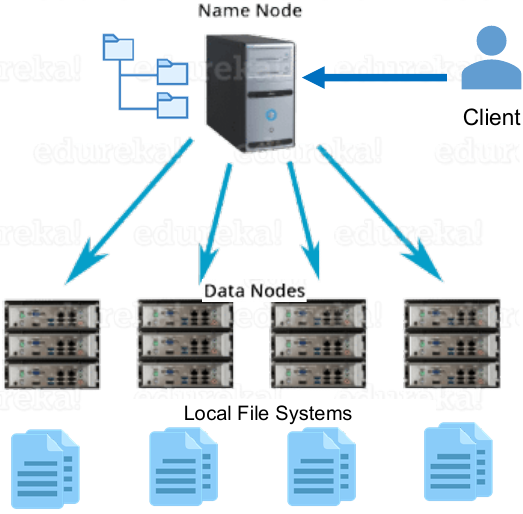
\includegraphics[scale=0.35]{figures/Schermata_20260603_153438.png}
\end{figure}

\subsection{Rapporto Manager Worker}
L'architettura manager-worker è un modello in cui un singolo nodo (o processo) manager coordina e gestisce più nodi (o processi) worker che eseguono le effettive attività di calcolo o di elaborazione dei dati.

Il nodo manager assegna i compiti ai worker e può anche occuparsi dall'aggregazione dei risultati

\begin{figure}[H]
    \centering
    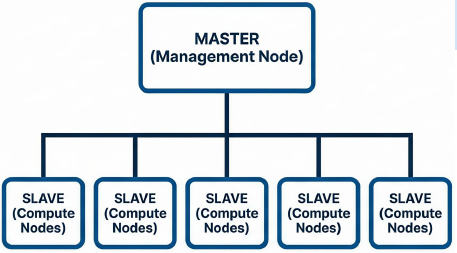
\includegraphics[scale=0.75]{figures/Schermata_20260603_153933.png}
\end{figure}

\subsection{Architetura hdfs}
HDFS ha un'architettura manager-worker

\begin{itemize}
    \item Un cluster HDFS è composto da un singolo NameNode, un server mangare che gestisce il namespace del file system e regola l'accesso ai file da parte dei client
    \item Sono presenti più DataNode, che gestiscono i volumi di archiviazione collegati ai nodi su cui sono in esecuzione
\end{itemize}

HDFS espone un unico file system per l'intero cluster e permette di memorizzare i dati utente in file all'interno dei DataNode.

Internamente, un file viene suddiviso in uno o più blocchi a questi vengono memroizzati in un insieme di DataNode (i chunk vengono replicati perdefaul 3 volte) 

\begin{figure}[H]
    \centering
    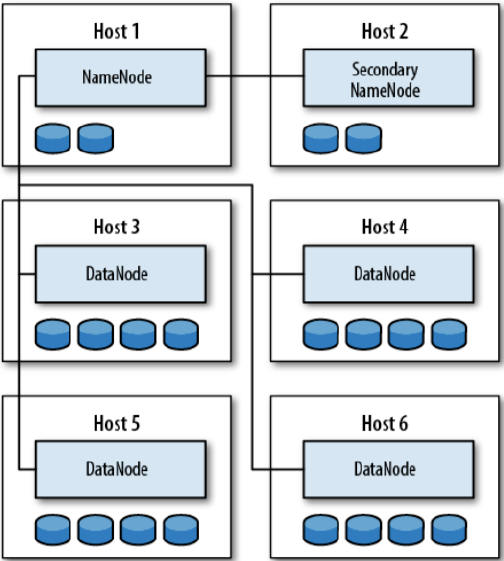
\includegraphics[scale=0.6]{figures/Schermata_20260603_154424.png}
\end{figure}

\begin{itemize}
    \item \textbf{NameNode}: Esegue le operazione sul file system come apertura, chiusura e rinomina di file e directory, inoltre determina la mappatura dei blocchi sui DataNode
    \begin{itemize}
        \item \uline{Gestione del file system}
        \begin{itemize}
            \item Mantiene i metadati della struttura di file e directory, la mappatua file-blocco, i permessi di accesso, ecc
        \end{itemize}
        \item \uline{Coordinamento delle operazioni sui file}
        \begin{itemize}
            \item Indirizza i client verso i DataNode per le operazioni di lettura e scrittura
            \item Infatti, nessun data transita attraverso il NameNode
        \end{itemize}
        \item \uline{Gestione dello stato di salute complessivo}
        \begin{itemize}
            \item Comunicazione periodica con i DataNode (health check)
            \item Replica e ribilanciamento dei blocchi
        \end{itemize}
    \end{itemize}
    \item \textbf{DataNode}: Sono responsabili di servire le richieste di lettura e scritta dei client oltre a creare, cancellare e replicare dei blocchi su istruzione del NameNode
    \begin{itemize}
        \item \underline{Block Server}
        \begin{itemize}
            \item Memorizza i dati nel file system locale
            \item Memorizza i metadati di un blocco
            \item Fornisce dati e metadati alle applicazioni client
        \end{itemize}
        \item \uline{Block Report}
        \begin{itemize}
            \item Perioticamente ina un report di tutti i blocchi esistenti al NameNode
        \end{itemize}
    \end{itemize}
\end{itemize}

\subsection{Creazione del file}
\begin{itemize}
    \item Il client calcola il checksum
    \item Il DataNode memorizza il checksum
\end{itemize}
\subsection{Accesso al file}
\begin{itemize}
    \item Il client recupera i dati e il checksum dal DataNode
    \item Se la validazione fallisce, il client tenta con altre replice
\end{itemize}

\newpage
\subsection{Replica dei dati}
HDFS è progettato per memorizzare in modo affidabile file di dimensioni molto grandi distributi su macchine in un grande cluster:
\begin{itemize}
    \item Memorizza ogni file come una sequenza di blocchi
    \item I blocchi di un file vengono replicati per garantire fault tolerance e prestazioni
\end{itemize}

\begin{figure}[H]
    \centering
    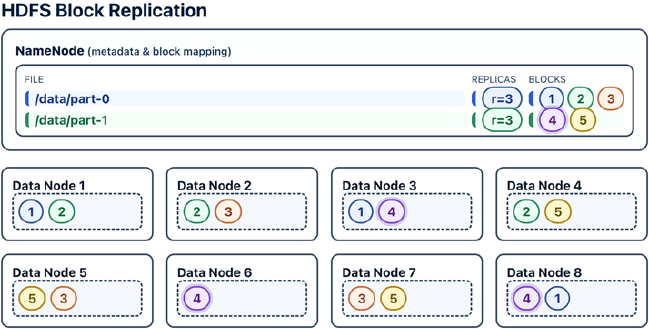
\includegraphics[scale=0.6]{figures/Schermata_20260604_105537.png}
\end{figure}

La dimensione del blocco e il fattore di replica sono configurabili per ogni singolo file:
\begin{itemize}
    \item Tutti i blocchi di un file, tranne l'ultimo, hanno la stessa dimensione
    \item Il fattore di replica può essere specificato al memomento della creazione del file e modificato successivamente (ribilanciamento)
\end{itemize}

\subsection{Forme della trasparenza}
\begin{table}[htbp]
\centering
\begin{tabularx}{\textwidth}{l c X}
\toprule
\textbf{Trasparenza} & \textbf{Implementata} & \textbf{Come in HDFS} \\
\midrule
Accesso & Sì & API uniforme (\texttt{FileSystem}, \texttt{hdfs://}): l'utente legge/scrive file ignorando rete e formato dei blocchi sottostanti. \\
\addlinespace
Posizione & Sì & Path logici (\texttt{/user/...}); il \texttt{NameNode} mappa ogni file ai \texttt{DataNode} che ospitano i blocchi. \\
\addlinespace
Rilocazione & No & HDFS è write-once: i blocchi di un file aperto non vengono spostati durante l'uso. \\
\addlinespace
Migrazione & Parziale & Il \texttt{Balancer} ridistribuisce i blocchi tra \texttt{DataNode} a riposo, in modo trasparente al client. \\
\addlinespace
Replica & Sì & Ogni blocco replicato (default $3\times$) su nodi/rack diversi; il client vede un solo file logico. \\
\addlinespace
Concorrenza & Limitata & Single-writer/multi-reader: più letture parallele, una sola scrittura per volta (lease del \texttt{NameNode}). \\
\addlinespace
Guasti & Sì & Heartbeat + ri-replica automatica dei blocchi; HA \texttt{NameNode} con standby. \\
\bottomrule
\end{tabularx}
\end{table}

\newpage
\section{YARN - Yet Another Resource Negotiator}
\subsection{Cosa è?}
Apache YARN è un software che gira su un gruppo di macchine e le condivide in modo equo tra molti programmi.

Decide quanta potenza di calcolo assegnare a ciascun programma, avvia e monitora i programmi durante l'esecuzione e impedisce che un programma rallenti o blocchi gli altri.

YARN può eseguire motli tipi di workload:
\begin{itemize}
    \item job batch
    \item streaming
    \item servizi e machine learning
\end{itemize}

\subsection{Cosa fa?}
È un motore che nasconde i complessi dettagli della gestione a runtime:
\begin{itemize}
    \item Parallelizzazione
    \item Load balancing
    \item Ottimizzazione dei trasferimento su disco
    \item Gestione dei guasti delle macchine
\end{itemize}

\subsection{Architetura}
Un \textbf{Resource Manager globale}:
\begin{itemize}
    \item Implementa uno scheduler globale delle risorse
    \item Assegna blocchi di risorse alle applicazioni richiedenti
    \item Le risorse provengono dai \textbf{NodeManager} (Worker)
    \item Arbitra le risorse tra applicazioni
\end{itemize}

Più \textbf{NodeManager}:
\begin{itemize}
    \item Ruolo di worker
    \item Comunica con il ResourceManager
    \item Gestisce le risorse locali
    \item Esegue (i task delle) applicazioni
\end{itemize}

\newpage
\subsection{Container}
\begin{tcolorbox}[title={Disclaimer}]
    I container YARN sono diversi dai container Docker/Linux.

    Non è coinvolta alcuna virtualizzazione: i container YARN rappresentano l'assegnazione di risorse ai task
\end{tcolorbox}

Rappresentano la logica delle risorse:
\begin{itemize}
    \item Creati \underline{su richiesta del ResourceManager}
    \item Riservano una certa quantità di risorse su un nodo
    \item Le applicazioni vengono eseguito in uno o più container
\end{itemize}

Quando viene sottomessa un'applicazione YARN, viene avviato un Application Master che ne supervisione l'esecuzione.

Negozia le risorse con il YARN Resource Manager e monitora l'esecuzione dei task

Un \textbf{Application Master} per ogni applicazione compatibile con YARN:
\begin{itemize}
    \item Uno per applicazione
    \item Viene eseguito in un container
    \item Richiede ulteriori container per eseguire i \textbf{task}
    \begin{itemize}
        \item Un task svolge una porzione specificato di lavoro, come l'elaborazione di un sottoinsieme di dati in un job MapReduce
    \end{itemize}
\end{itemize}

\subsection{Forme di trasparenza}
\begin{table}[htbp]
\centering
\begin{tabularx}{\textwidth}{l c X}
\toprule
\textbf{Trasparenza} & \textbf{Implementata} & \textbf{Come in YARN} \\
\midrule
Accesso & Sì & API uniformi (\texttt{ApplicationMaster}, \texttt{ResourceManager}) per richiedere risorse: il client sottomette job ignorando dove gireranno i container. \\
\addlinespace
Posizione & Sì & Il \texttt{ResourceManager} assegna i container ai \texttt{NodeManager}; l'applicazione interagisce con risorse logiche, non con host fisici. \\
\addlinespace
Rilocazione & No & Un container in esecuzione non viene spostato: in caso di fallimento del nodo viene riavviato altrove (\textit{preemption}, non migrazione live). \\
\addlinespace
Migrazione & No & YARN non sposta task attivi tra nodi; il riavvio comporta perdita dello stato locale del container. \\
\addlinespace
Replica & Parziale & Repliche solo dei componenti di sistema (HA del \texttt{ResourceManager} con standby); i container applicativi non sono replicati. \\
\addlinespace
Concorrenza & Sì & Scheduler (Capacity/Fair) gestisce richieste concorrenti di più applicazioni e utenti, isolando risorse via queue e \texttt{cgroups}. \\
\addlinespace
Guasti & Sì & \texttt{NodeManager} heartbeat + retry automatico dei container falliti; \texttt{ApplicationMaster} recovery; HA del \texttt{ResourceManager}. \\
\bottomrule
\end{tabularx}
\end{table}

\subsection{Esecuzione di un'applicazione}
\begin{enumerate}
    \item Quando un applicazione YARN viene sottomessa, viene avviato un \textbf{Application Master} per supervisionare l'esecuzione dell'applicazione stessa.

    Negozia le risorse con il Resource Manager di YARN e monitora l'esecuzione dei task.

    Un task esegue una porzione specifica di lavoro, ad esempio l'elaborazione di un sottoinsieme di dati in un job MapReduce

    \begin{figure}[H]
        \centering
        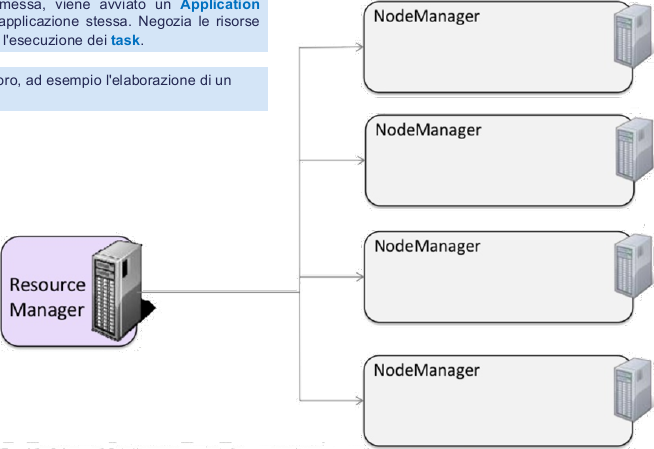
\includegraphics[scale=0.5]{figures/Schermata_20260604_112322.png}
    \end{figure}

    \item Il client sottomette un'applicazione compatibile con YARN

    Il RM alloca un container e avvia l'Application Master

    \begin{figure}[H]
        \centering
        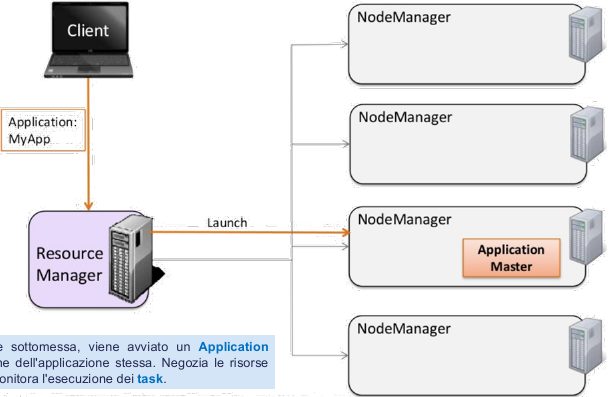
\includegraphics[scale=0.5]{figures/Schermata_20260604_112646.png}
    \end{figure}

    \begin{tcolorbox}
        Quando un'applicazione YARN viene sottomessa, viene avviato un Application Master per supervisionare l'esecuzione dell'applicazione stessa.

        Negozia le risorse con il Resource Manager di YARN e monitora l'esecuzione dei task
    \end{tcolorbox}
    
    \newpage
    \item L'Application Master richiede i container al Resource Manager

    \begin{figure}[H]
        \centering
        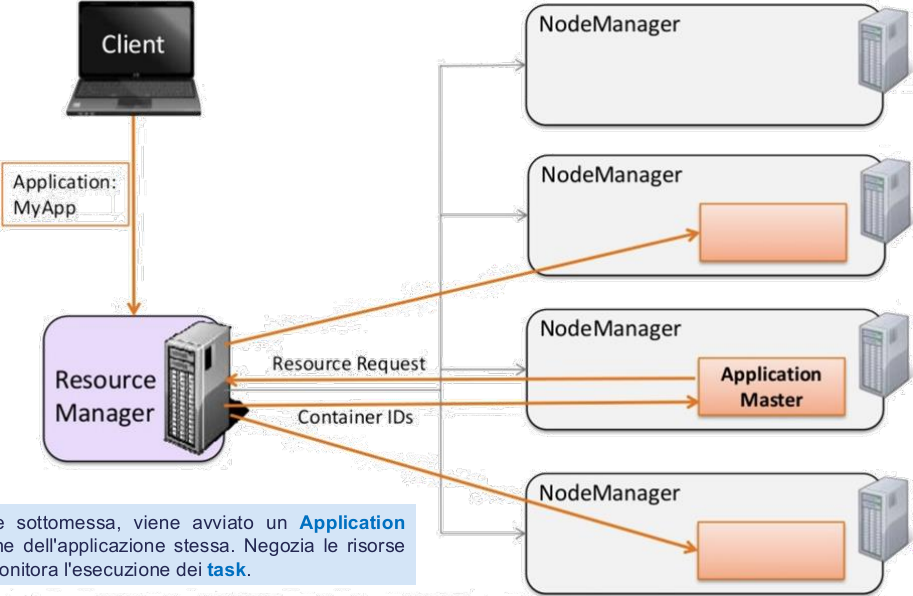
\includegraphics[scale=0.4]{figures/Schermata_20260604_112838.png}
    \end{figure}

    \item L'Application Master schedula i task dell'applicazione sui container
    \begin{figure}[H]
        \centering
        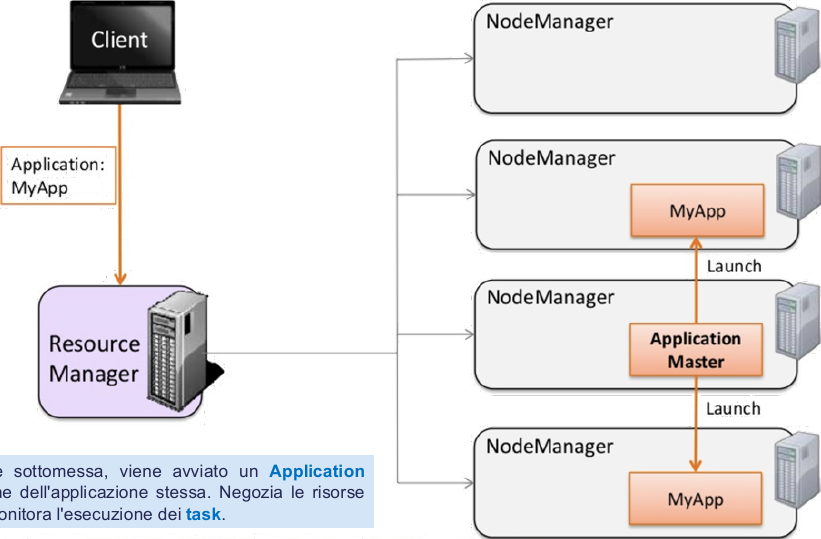
\includegraphics[scale=0.4]{figures/Schermata_20260604_113040.png}
    \end{figure}

    \item Il cluster è multi-tenant

    Il \textbf{Resource Manager} può gestire più applicazioni grazie alle proprie politiche di allocazione

    \begin{figure}[H]
        \centering
        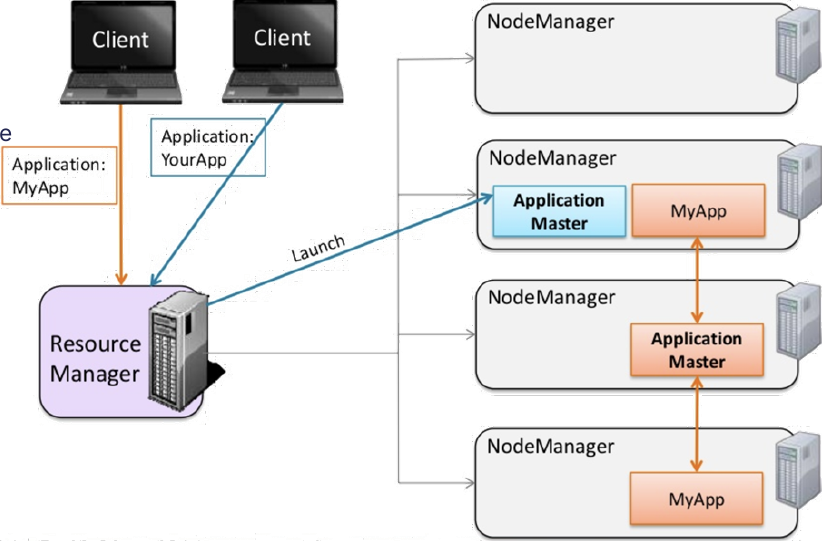
\includegraphics[scale=0.5]{figures/Schermata_20260604_113332.png}
    \end{figure}

    \newpage
    \begin{figure}[H]
        \centering
        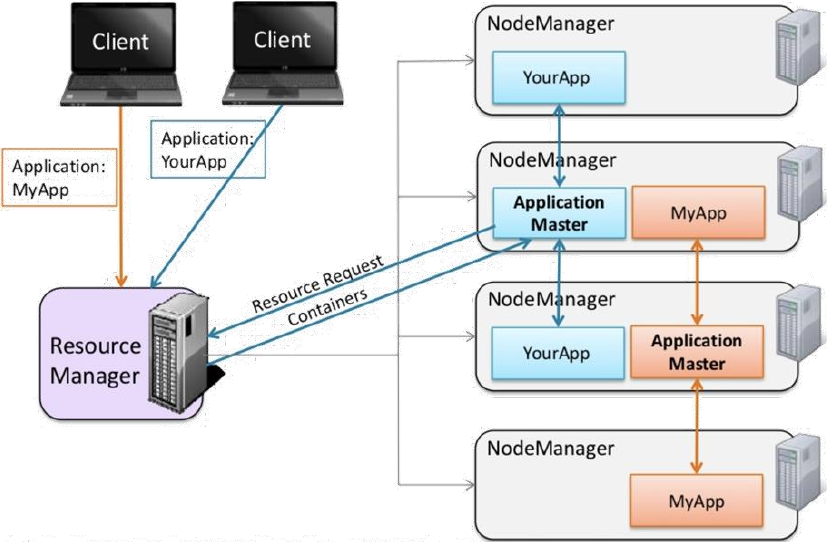
\includegraphics[scale=0.5]{figures/Schermata_20260604_114513.png}    
    \end{figure}
\end{enumerate}

\section{Data locality in YARN + HDF}
\begin{tcolorbox}
    Quando un applicazione YARN (per esempio creata con la libreria MapReduce) viene sottomessa, viene avviato un \textbf{Application Master} per supervisionare l'esecuzione dell'applicazione stessa.

Negozia le risorse con il Resource Manager di YARN e monitora l'esecuzione dei task
\end{tcolorbox}

\begin{enumerate}
    \item Notare che un NodeManager e un DataNode dovrebbero risiedere sullo stesso nodo
    \begin{figure}[H]
        \centering
        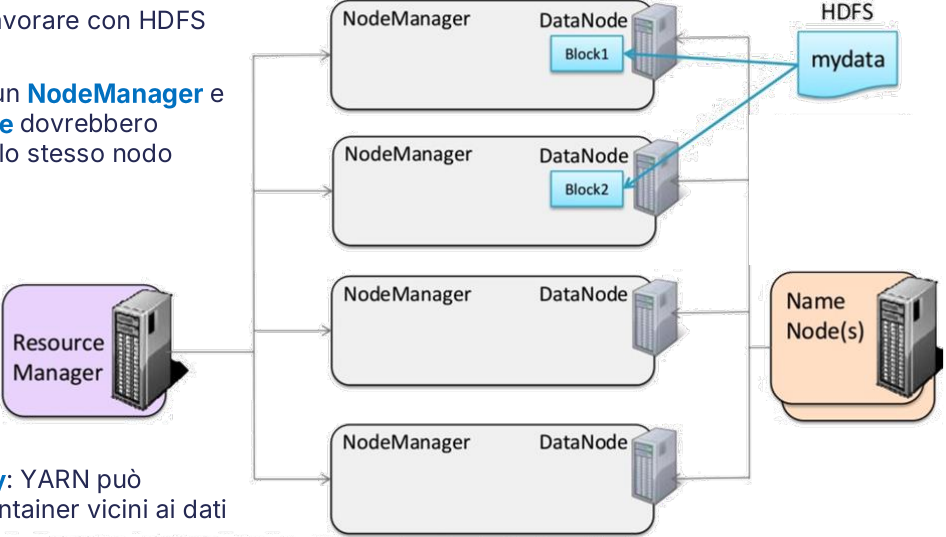
\includegraphics[scale=0.5]{figures/Schermata_20260604_115352.png}
    \end{figure}

    \newpage
    \item 
    \begin{figure}
        \centering
        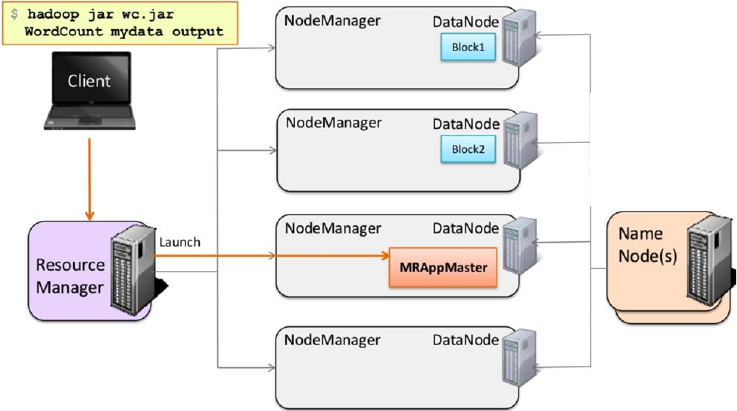
\includegraphics[scale=0.6]{figures/Schermata_20260604_115452.png}
    \end{figure}

    \item 
    L'ApplicationMaster usa i metadati di HDFS (come la posizione dei blocchi) per determinare dove risiedono i dati
    \begin{figure}[H]
        \centering
        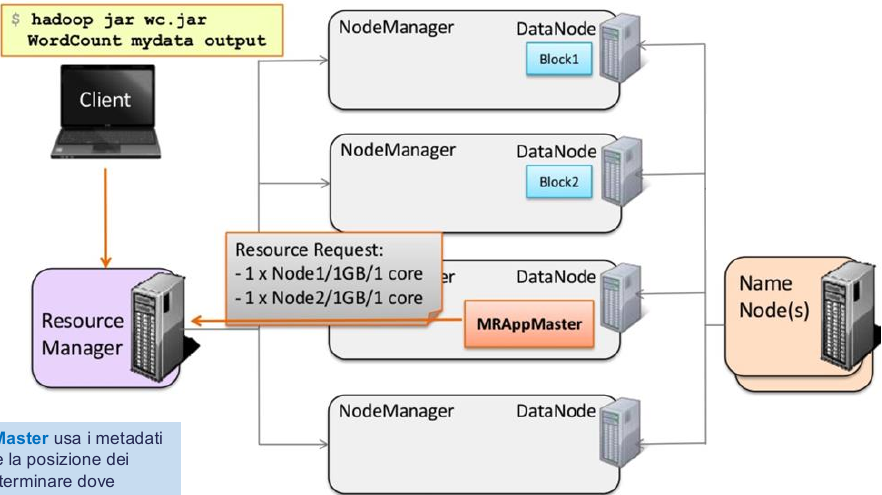
\includegraphics[scale=0.6]{figures/Schermata_20260604_115627.png}
    \end{figure}

    \item 
    \begin{figure}[H]
        \centering
        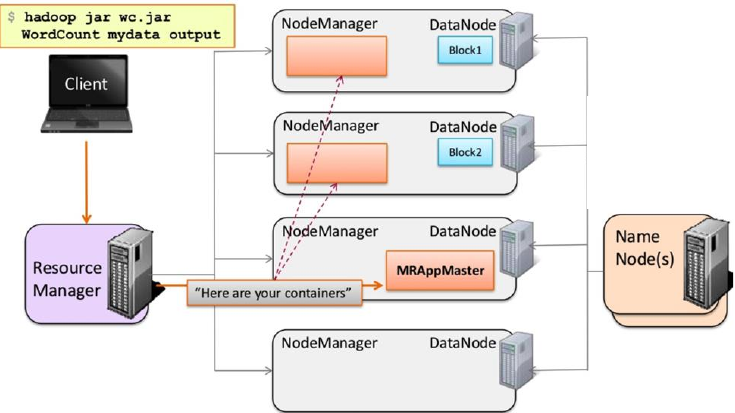
\includegraphics[scale=0.5]{figures/Schermata_20260604_115810.png}
    \end{figure}

    \item 
    \begin{figure}
        \centering
        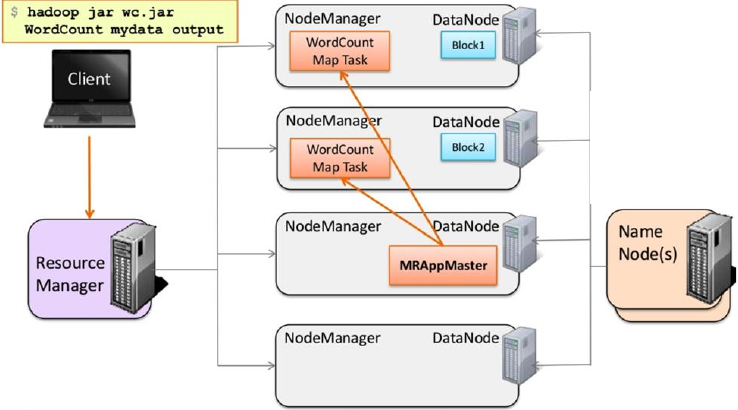
\includegraphics[scale=0.5]{figures/Schermata_20260604_115919.png}
    \end{figure}

    \item 
    I Map Task generano risultati parziali in un buffer in memoria oppure sul disco locale del nodo dove il Map task è in esecuzione i dati non vengono scritti su HDFS perchè sono transitori e non necessitano di replicazione

    \begin{figure}[H]
        \centering
        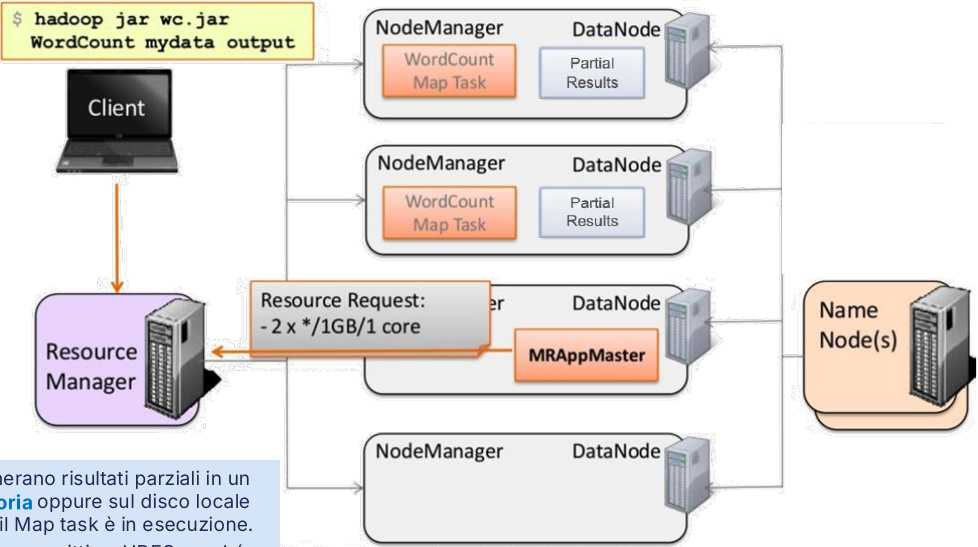
\includegraphics[scale=0.5]{figures/Schermata_20260604_120117.png}
    \end{figure}

    \item 
    L'ApplicationMaster richiede risorse per allocare i Reduce task
    \begin{figure}[H]
        \centering
        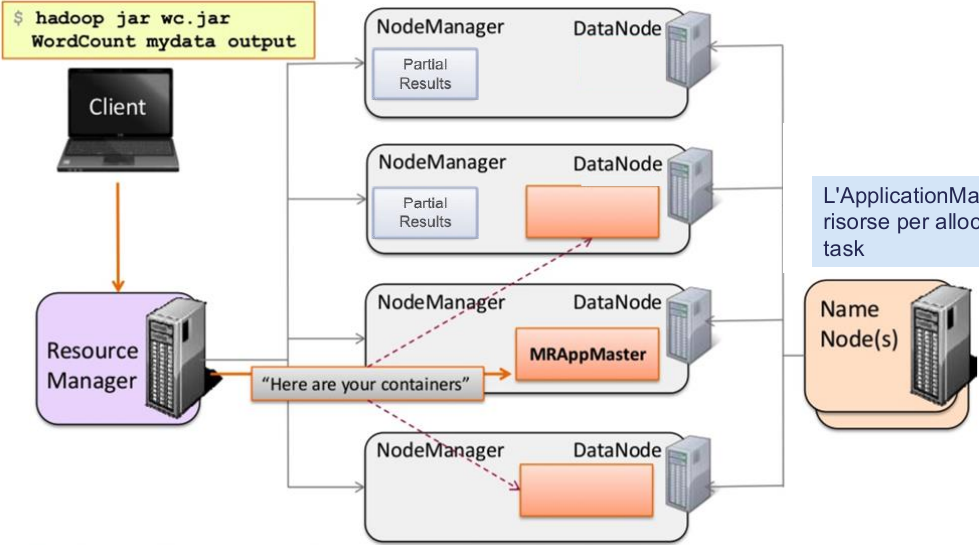
\includegraphics[scale=0.5]{figures/Schermata_20260604_120253.png}
    \end{figure}

    \newpage
    \item I Reduce Task consumano i risultati parziali prodotti dai Map Task.

    I dati vengono ordinati e raggruppati per chiave prima di essere passati alla funzione reduce
    \begin{figure}[H]
        \centering
        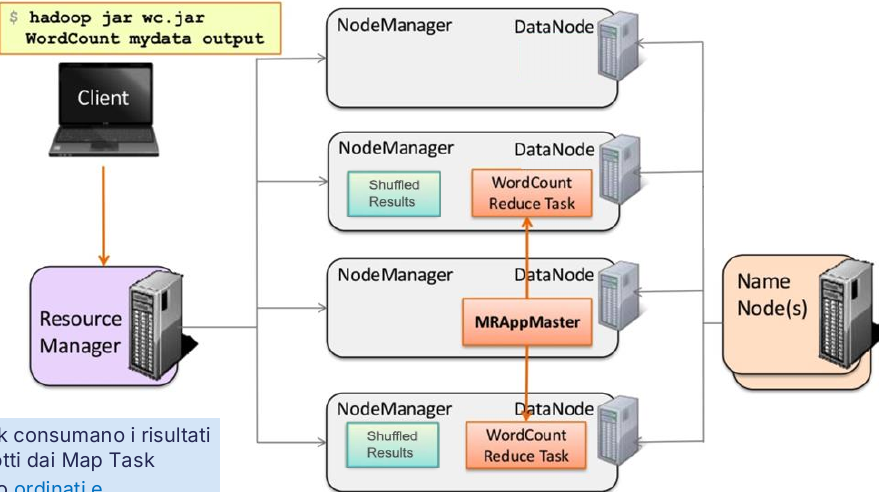
\includegraphics[scale=0.5]{figures/Schermata_20260604_120455.png}
    \end{figure}

    \item 
    I risultati finali possono essere restituiti al client o scritti su HDFS.
    \begin{figure}[H]
        \centering
        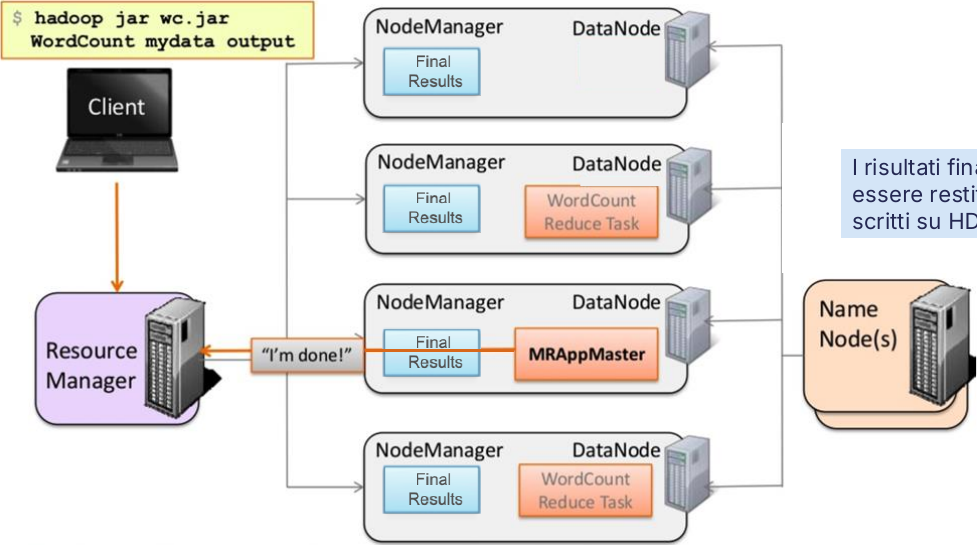
\includegraphics[scale=0.5]{figures/Schermata_20260604_120613.png}
    \end{figure}
\end{enumerate}



